\chapter{Architektura systemu}

\section{Komponenty}

\begin{itemize}
  \item Kontroler rozpoznawania pojazdów
  \item Szlaban - oparty na systemie wbudowanym
  \item Kontroler przejazdu - odpowiada za utrzymanie sesji. Upewnia się, że szlaban jest zawsze w takiej pozycji jakiej powinien
  \item Kontroler płatności
  \item Baza danych
  \item Operator - reprezentuje funkcjonalnośći administratora/operatora
\end{itemize}

\begin{figure}[H]
	\centering
  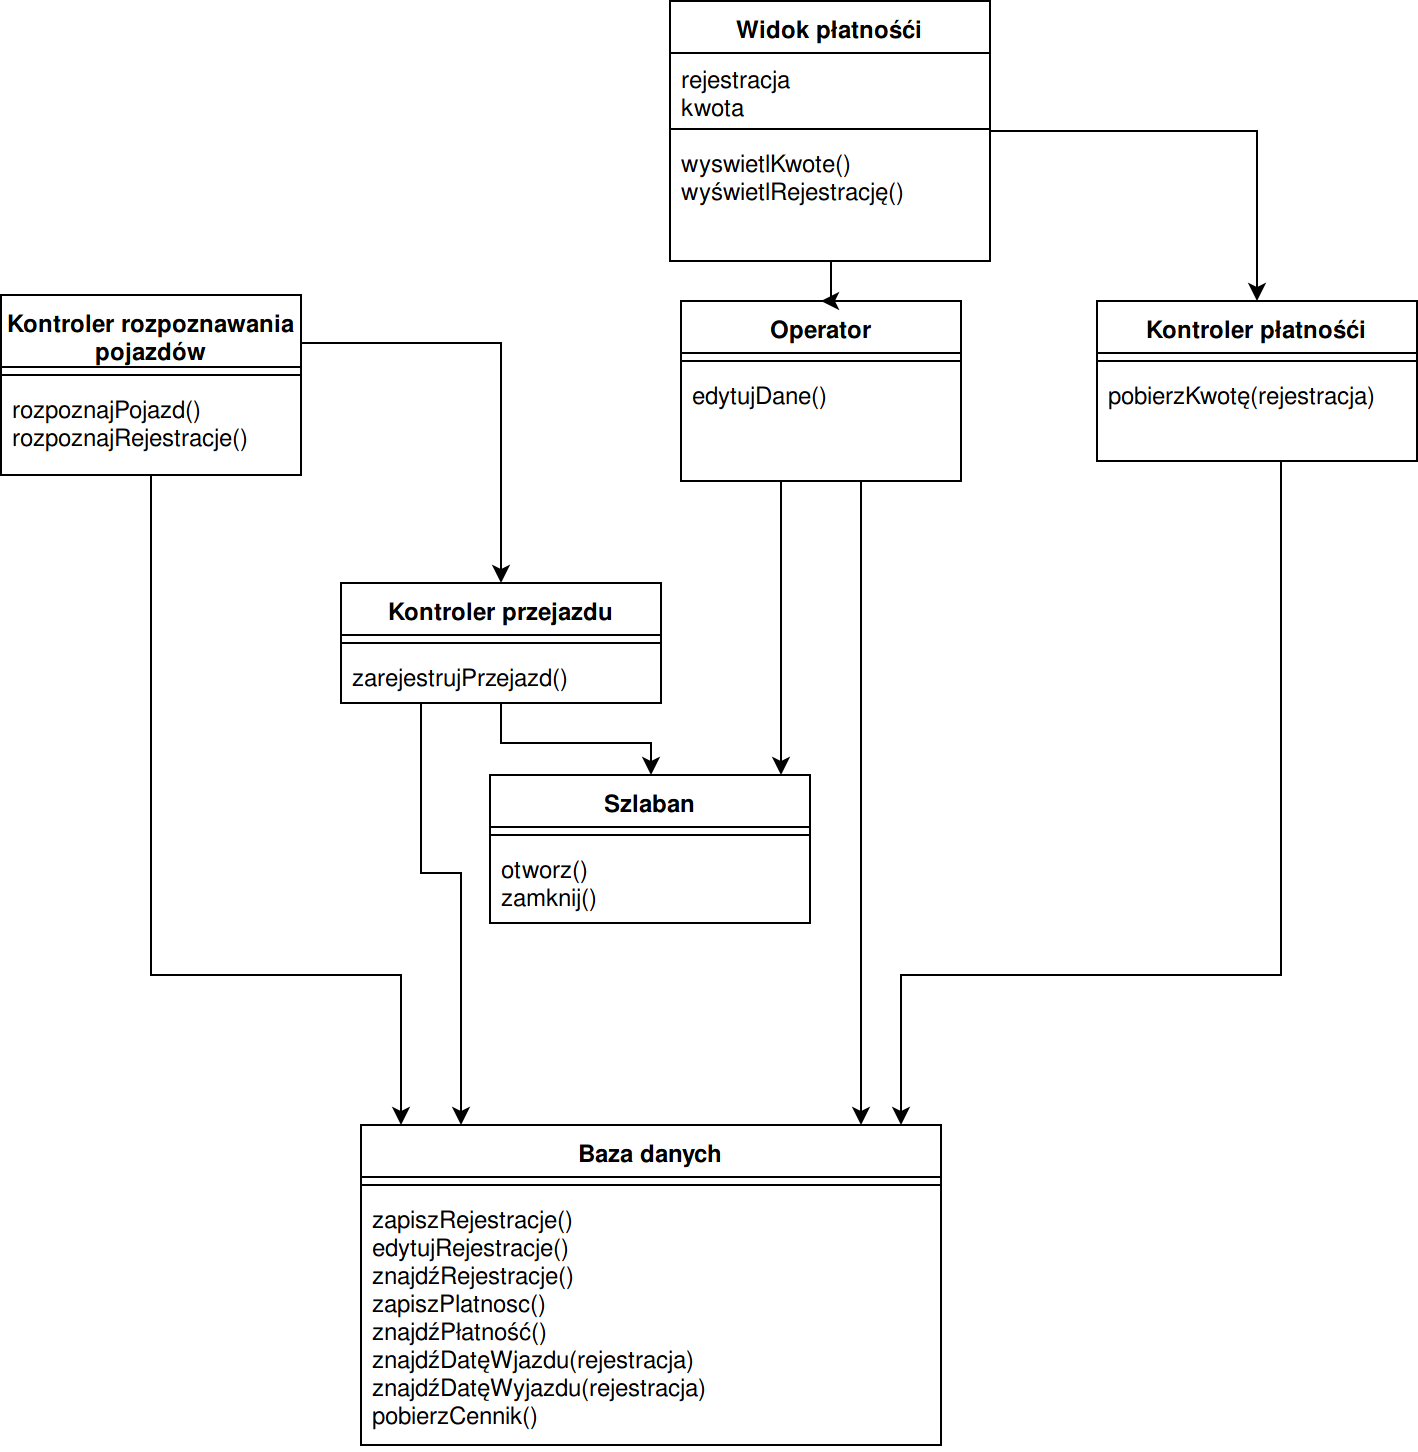
\includegraphics[width=100mm]{diagramy/komponentyZaleznosci.png}
  \caption{Zależności między komponentami}
\end{figure}

\begin{figure}[H]
	\centering
	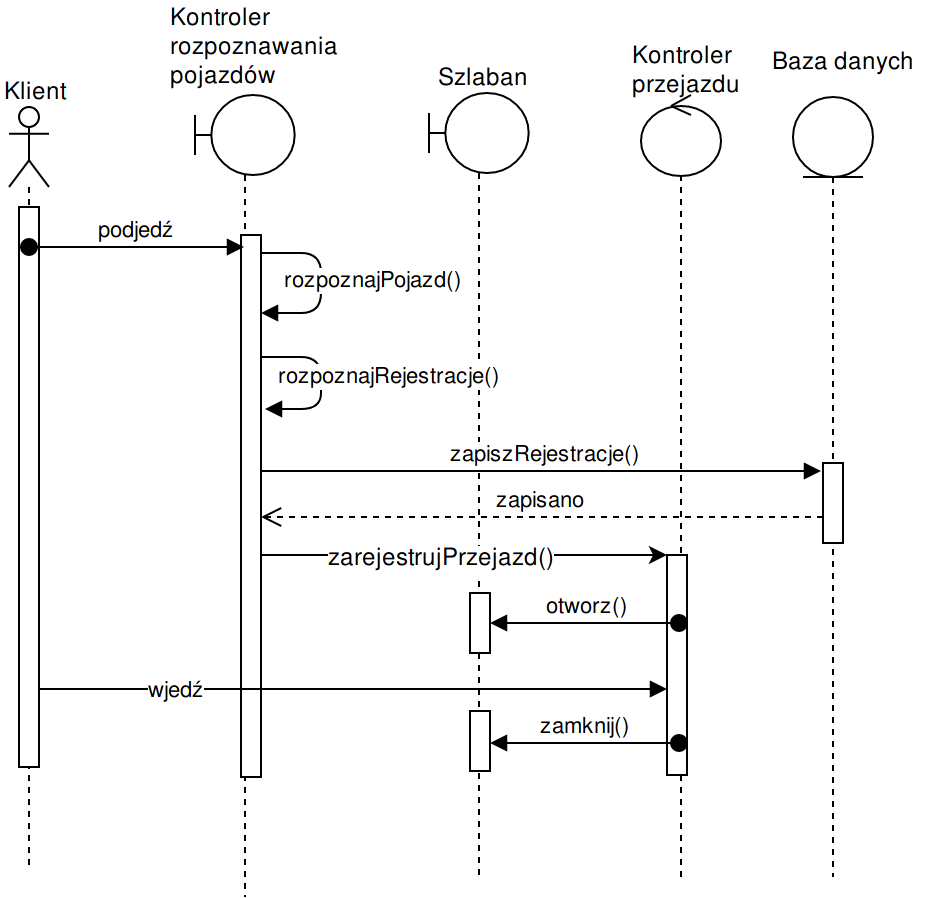
\includegraphics[width=100mm]{diagramy/sekwencyjnyWjazd.png}
	\caption{Diagram sekwencji dla przypadku użycia UC1 - wjazd z parkingu}
\end{figure}

\begin{figure}[H]
	\centering
	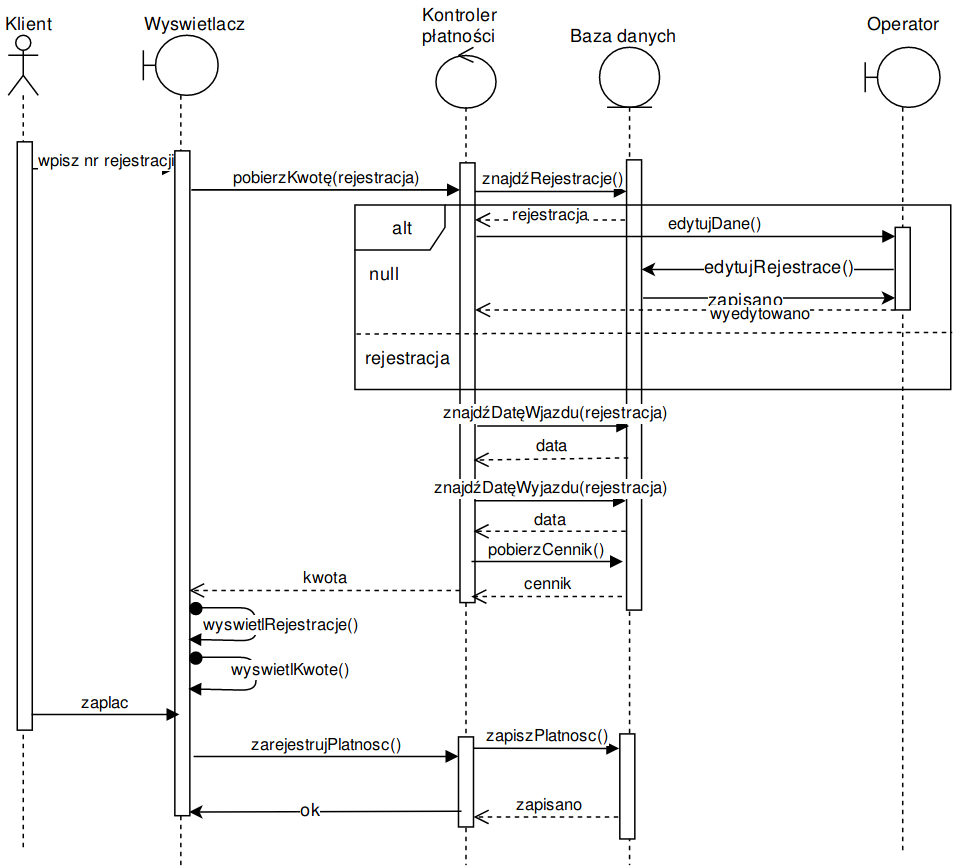
\includegraphics[width=100mm]{diagramy/sekwencyjnyPlatnosci.png}
  \caption{Diagram sekwencji dla przypadku użycia UC3 - obsługa terminala}
\end{figure}

\begin{figure}[H]
	\centering
	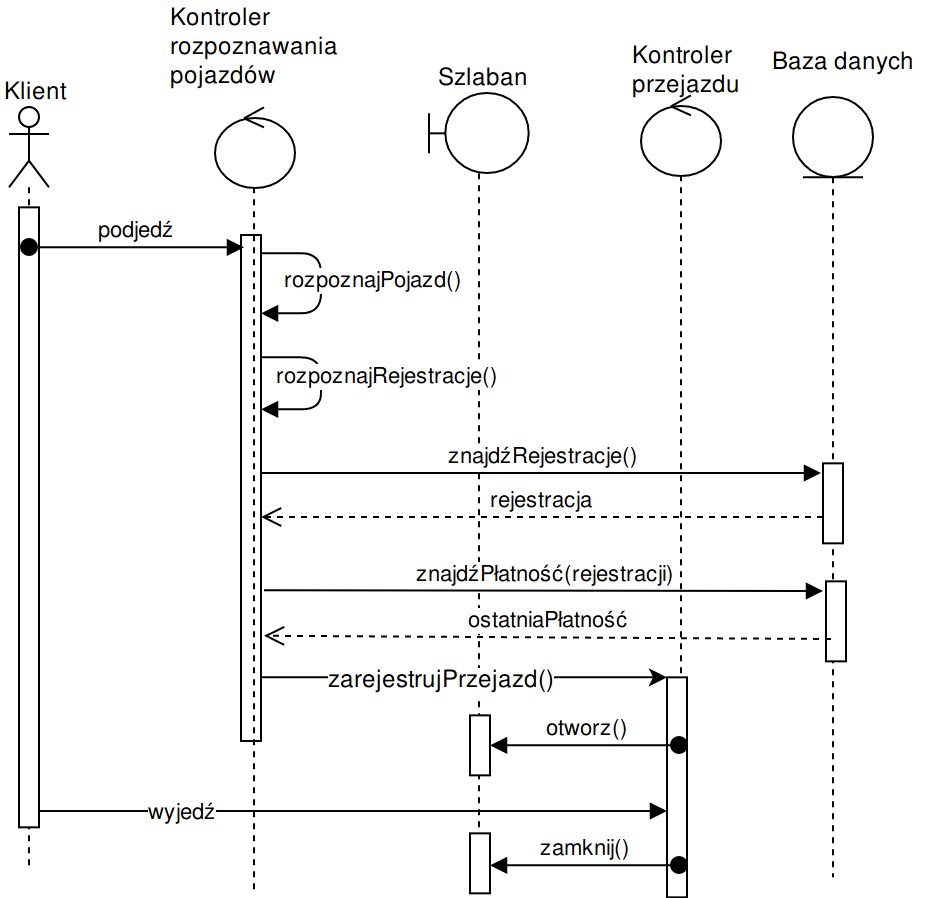
\includegraphics[width=100mm]{diagramy/sekwencyjnyWyjazd.png}
  \caption{Diagram sekwencji dla przypadku użycia UC5 - wyjazd z parkingu}
\end{figure}



